\begin{frame}{Características do Hyperledger Fabric}

	\begin{itemize}
		\item \textbf{Permissão de Acesso:} Rede blockchain permissionada, onde os
		      participantes precisam de identidade verificada.
		\item \textbf{Modularidade:} Suporte a diferentes mecanismos de consenso,
		      gerenciamento de identidade e banco de dados de estado.
		\item \textbf{Arquitetura Flexível:} Separação entre nós de execução
		      (\textit{peers}) e de ordenação (\textit{orderers}).
		\item \textbf{Chaincodes:} Contratos inteligentes executados fora do nó de
		      consenso, melhorando a escalabilidade.
		\item \textbf{Alta Escalabilidade:} Suporte a múltiplas organizações, canais
		      e modelos de governança distribuída.
		\item \textbf{Desempenho e Eficiência:} Modelo sem mineração, resultando em
		      menor latência e maior eficiência.
	\end{itemize}

\end{frame}

\begin{frame}{Algoritmo de Consenso Raft}

	\begin{itemize}
		\item Raft é um algoritmo de consenso projetado para gerenciar um log
		      replicado de forma confiável~\cite{raft}.
		\item O algoritmo opera elegendo um líder, que coordena a replicação de logs
		      entre os servidores~\cite{ongaro2014raft}.
		\item O líder recebe entradas de log dos clientes, propaga para os
		      seguidores e garante que os registros sejam aplicados com segurança.
		\item Caso o líder falhe ou se desconecte, um novo líder é escolhido através
		      de um processo de eleição.
		\item Raft divide o problema de consenso em três partes:
		      \begin{itemize}
			      \item \textbf{Eleição de líder}: Escolha de um novo líder quando
			            necessário~\cite{ongaro2014raft}.
			      \item \textbf{Replicação de log}: Garantia de consistência entre os
			            servidores.
			      \item \textbf{Segurança}: Prevenção de registros inconsistentes ou
			            inválidos.
		      \end{itemize}
	\end{itemize}

\end{frame}

\begin{frame}{Visualização Raft}

	\begin{figure}
		\centering
		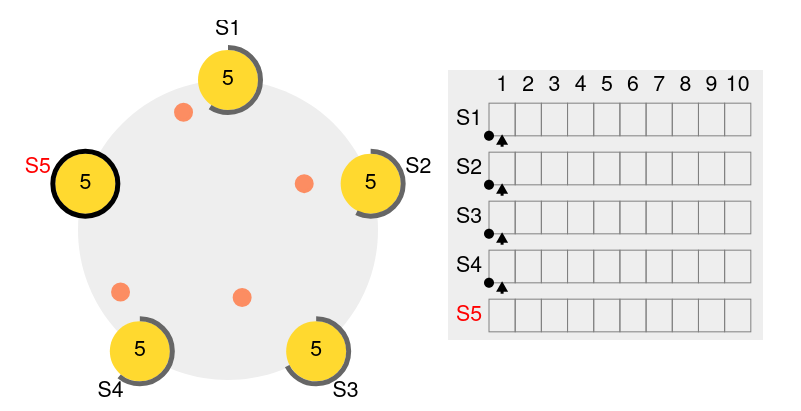
\includegraphics[width=0.8\textwidth]{figures/raftvisualization.png}
		\caption{Visualização de consenso Raft.\ \textit{Fonte:~\cite{raftscope}}.}
		\label{fig:raftvisualization}
	\end{figure}

\end{frame}

\begin{frame}{Elementos de uma Rede Fabric}

	\begin{itemize}
		\item \textbf{Certificate Authorities (CAs):} Emitem e gerenciam identidades
		      na rede via certificados X.509.
		\item \textbf{Ledgers:} Livro-razão composto pelo \textit{Blockchain}
		      (histórico de transações) e \textit{State Database} (estado atual).
		\item \textbf{Channels:} Criam redes privadas para transações isoladas e
		      seguras.
		\item \textbf{Ordering Services:} Ordenam e distribuem transações em blocos,
		      garantindo consistência.
	\end{itemize}

\end{frame}

\begin{frame}{Elementos de uma Rede Fabric}

	\begin{itemize}
		\item \textbf{Peers:} Nós que armazenam o ledger e executam
		      \textit{chaincodes}. Tipos:
		      \begin{itemize}
			      \item \textbf{Endorsing Peers:} Validam e simulam transações.
			      \item \textbf{Committing Peers:} Aplicam blocos ao ledger.
			      \item \textbf{Anchor Peers:} Facilitam comunicação entre
			            organizações.
		      \end{itemize}
		\item \textbf{Organizations:} Empresas/instituições com seus próprios
		      \textit{peers} e regras.
		\item \textbf{Chaincodes:} Contratos inteligentes que processam transações e
		      alteram o ledger.
		\item \textbf{Clients:} Aplicações que enviam transações, coletam aprovações
		      e as submetem à rede.
	\end{itemize}

\end{frame}

\begin{frame}{Rede Fabric}

	\begin{figure}
		\centering
		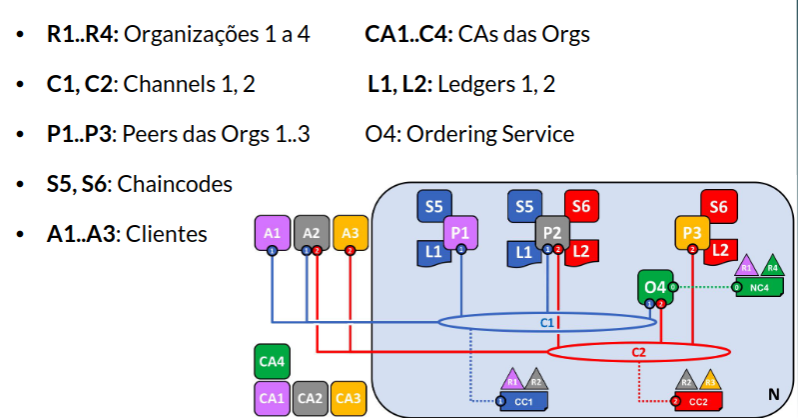
\includegraphics[width=0.8\textwidth]{figures/fabricexample.png}
		\caption{Exemplo de rede Fabric.\ \textit{Fonte: Escola Superior de Redes}.}
		\label{fig:fabricexample}
	\end{figure}

\end{frame}
